%\enlargethispage*{2cm}

\paragraph{Research Team}
 Ursula M. Staudinger (Professor of Psychology), Ben Godde (Professor of Neuroscience), Heike Heidemeier (Postdoctoral fellow, Psychology), Brigitte Kudielka-W�st (Professor of Health Psychology), Christian Rossnagel (Professor of Organizational Behavior), Klaus Sch�mann (Professor of Sociology), Mireille Trautmann (Postdoctoral Fellow, Neuroscience), Claudia Voelcker-Rehage (Lecturer, Human Performance), Sven V�lpel (Professor of Business Administration), Stefan Baron (Doctoral Fellow, Sociology), Catherine Bowen (Doctoral Fellow, Psychology), Nicolas Feuerhahn (Doctoral Fellow, Health Psychology), Daniela Noethen (Doctoral Fellow, Business Administration).

\null
\textbf{Description of the project\smallskip}


Demographic change challenges management and corporate strategies as well as aging individuals. Companies face the challenge of staying innovative and productive with fewer young talents on the labor market, while individuals need to frequently update their skills and knowledge to maintain high levels of employability into (statutory) retirement age. Above all, employees' physical and psychological health is an invaluable resource and a precondition for the ability to maintain high levels of productivity throughout a career. Since the impact of demographic change on organizations is multifaceted, and demands action in several fields, an interdisciplinary perspective on productive aging is fitting.  All JCLL professors have worked together to contribute diverse perspectives within a joint research project. Project "Demopass" (from the German words "Demografie" and "Passung": demography and match/mismatch) examines matches and mismatches between several organizational levels (employees, management, and organizational strategies) that are crucial for understanding organizational outcomes, such as employee health and productivity. Moreover, the project emphasizes the important role that organizational climate (an aspect of an organization's social capital) plays in understanding organizational outcomes. Organizational climate communicates (implicit) expectations, values and incentives that may have a marked influence on actual behavior and the success of organizational strategies. The concept of matches and mismatches between three perspectives defines a reference framework that guides the work of five subprojects. 



\begin{figure}[htp]
 \begin{center}
    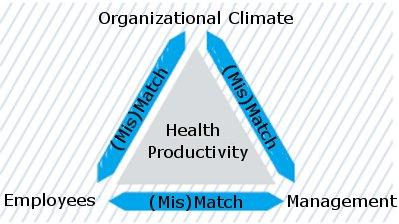
\includegraphics[natwidth=150, natheight=100]{fig1.jpg}
    \caption{Project Demopass}\label{fig:fig1}
   \end{center}
\end{figure}


%insert picture
%insert picture
%insert picture


\textbf{Research objectives}
 Project "Demopass" identifies five fields of action that are specifically relevant to tackling the challenges posed by demographic change in organizations: intergenerational knowledge transfer, training and on-the-job learning, images of aging in organizations, adaptive competences, and physical as well as psychological health. Exemplary research questions include the following: In order to establish successful knowledge management, employees' abilities to communicate and seek knowledge must match the expectations, resources and support provided by supervisors, as well as the forces implied in organizational climate. Specific consideration is given to intergenerational ("young to old" and "old to young") knowledge transfer. Similarly, images of aging and age-related organizational policies must be communicated in ways so that they match the beliefs of both employees and their supervisors. A company's "age climate" determines how others perceive older workers, and conveys whether they are esteemed members of the organization. Negative stereotyping may impair the motivation and productivity of older workers. This applies to self-views as well as the (assumed) views of others. Indeed, personal views and the views of others (supervisor beliefs or shared beliefs; i.e. "age climate") may positively or negatively complement or compensate for one other. A positive "age climate" may particularly help employees who tend to think negatively about their own aging to maintain effective self-regulation and higher levels of productivity. As a final example, the subproject on adaptive competencies examines meta-competencies that are highly relevant (in addition to specific skill or expertise) to meeting work demands. Again, an important assumption is that a match between perceived work demands, actual demands, and also employees' adaptive competencies contributes to an understanding of physical health and psychological well-being at work. Having to meet excessive demands may be as detrimental as insufficient challenge of skill and adaptive competencies. For the remaining two fields, training and health psychology, the same framework is applied to study matches and mismatches among the employees' competencies or attitudes, management support and strategies, and work climate.

\smallskip
 By studying a number of "paralleling" research questions, the project seeks to contribute to current understanding, while implementing an interdisciplinary approach. But the project also aims to communicate results so they are able to inform management practice. For that purpose, participating companies will receive feedback about their results. In addition, the project will assemble a toolbox for diagnosing matches and mismatches in organizations; this will be made available to companies which then can independently employ it. 


\paragraph{Outlook} 
  By the end of 2008, the project "Demopass" will have finished with data collection in five partnering companies. The project will then have collected questionnaire data and indicators of objective health from roughly 1500 employees and their supervisors. In addition, interviews with management representatives provide information about corporate and work strategies.  The research questions will be addressed empirically using a multi-level design, with individuals sampled from their work teams in order to ensure that they share the same social and physical work environment and climate. 

 Research results will begin to come to fruition in 2009. The project team also plans to carry out another round of data collection in order to validate the previously mentioned toolbox. This will be structured as a shortened version of the original questionnaire that will be tailored to address essential aspects of match/mismatch in the five action fields, and that will be designed to be applied by practitioners. In 2010 the project will attempt to scale up outreach both within the scientific community and with other relevant actors in private and public organizations. 

\paragraph{Grant} 
 Grant sponsorship was provided by the BMBF and the European Social Fund, "Effects of Matches/Mismatches between Aspects of Human and Social Capital, Corporate Strategy and Work Organization on the Physical and Mental Well-Being of Employees" (April, 2007). 

 Competency models are widely used by Human Resource (HR) practitioners in the selection, placement and development of employees. However, only little competency modeling research has been conducted, and the issue of age-related competency changes has hardly ever been addressed. In collaboration with Bosch Rexroth AG, we are developing a competency model that incorporates employees' age-related changes in ability and motivation factors. The model is intended to help identify HR development requirements in the mid-term (5 years).


 
